

\setchapterpreamble[u]{\margintoc}
\chapter{Linear regression}
\label{chap:linear_regression}

We observe iid pairs $(X_1, Y_1), \ldots, (X_n, Y_n)$ where $X_i \in \R^d$ and $Y_i \in \R$.
We want to learn to \emph{predict} $Y_i$ from $X_i$, namely we want to \emph{regress} $Y_i$ on $X_i$.
We know that the closest $X_1$-measurable function which is the closest from $Y_1$ in $L^2$ is the conditional expectation $\E [Y_1 | X_1] = f(X_1)$ for some measurable function $f$, but we do not know the joint distribution of $(X_1, Y_1)$, so we don't know $f$.
Therefore, we want to use the observations $(X_i, Y_i)$ for $i=1, \ldots, n$ in order to build some approximation of $f$.

What kind of functions should we consider ?
We can consider the simplest non-constant function $\R^d \go \R$ that we can think of, which is naturally a \emph{linear} function $x \mapsto x^\top w + b$, hence the name \emph{linear regression model}.

\begin{kaobox}[frametitle=Features engineering]
	Considering only linear functions is of course very limiting. But let us stress that, in practice, we can do whatever we want with the data $(X_1, Y_1), \ldots, (X_n, Y_n)$. 
	A linear model is typically \emph{trained} on \emph{mappings} of $X_i$, that can include non-linear mappings, such as a \emph{polynomial mapping}, that includes all the pairwise products leading to $d(d-1)/2$ extra coordinates, etc.
	It is uncommon (and suspicious) to work directly with the \emph{raw} vectors of \emph{features} $X_1, \ldots, X_n$: a lot of effort is usually put on the construction of a mapping, that requires knowledge about the data itself.
	The construction of such a \emph{features mapping}%
	\marginnote[*-2]{The problem considered here is also known as an instance of \emph{supervised learning} with vectors of \emph{features} $X_i \in \R^d$ and \emph{labels} $Y_i \in \R$.}
	is called \emph{feature engineering} in statistics and machine learning, and is more an art than a science. 
	Many industrial large scale problems%
	\marginnote{Large scale means that both $n$ and $d$ are large, when $n$ is large and $n \gg d$ we are considering \emph{big data} while when $d$ is large and $d \gg n$ we work with \emph{high-dimensional} data.}
	(such as web-display advertisement) are handled using simple linear models, but on highly tested and engineered feature mappings. We won't discuss this in this chapter, and will assume that $X_i$ are well-crafted vectors of features on which we want to train a linear model.	
\end{kaobox}

\emph{Training} a linear model means \emph{learning} the \emph{model weights} $w \in \R^d$ and the \emph{intercept} or \emph{population bias} $b \in \R$.  
To simplify notations we will forget about the intercept from now on, since without loss of generality we can simply put $\theta = [1 \; w^\top]^\top$ and replace $X_i$ by $[1 \; X_i^\top]^\top$ (and $d$ by $d +1$).

\section{Ordinary least squares estimator} % (fold)
\label{sec:least_squares_estimator}

A linear model assumes that
\begin{equation*}
	Y_i = X_i^\top \theta  + \eps_i
\end{equation*}
for $i=1, \ldots, n$, where $\theta \in \R^d$ must be trained using the data $(X_1, Y_1), \ldots, (X_n, Y_n)$ and where the random variables $\eps_i$ are called \emph{noise}, and are assumed to satisfy $\E[\eps_i | X_i] = 0$.
Also, we will assume from now on that $(X_1, Y_1), \ldots, (X_n, Y_n)$ is iid.
Let us also consider an independent pair $(X, Y)$ with the same distribution.
We want to answer to the question:
how can we \emph{estimate} or \emph{train} $\theta$?
A natural idea is to find $\wh \theta_n \in \R^d$ such that $X_i^\top \wh \theta_n$ is close to $Y_i$ for each $i=1, \ldots, n$. 
The simplest way to measure this closeness is to use the Euclidean distance on $\R^n$.
Let us first introduce the vector of \emph{labels} $\by = [Y_1 \cdots Y_n]^\top \in \R^n$%
\marginnote{A vector in $\R^n$ is written as a column matrix with shape $n \times 1$ and the norm $\norm{\cdot}$ stands for the Euclidean norm. We will write inner products between same-shaped vectors as $u^\top v$ or $\inr{u, v}$ depending on what is more convenient.}
and the \emph{features} matrix
\begin{equation*}
	\bX = 
	\begin{bmatrix}
		X_{1, 1} & \cdots & X_{1, d} \\
		\vdots & \ddots & \vdots \\
		X_{n, 1} & \cdots & X_{n, d}
	\end{bmatrix}	
	=
	\begin{bmatrix}
		X_1^\top \\
		\vdots \\
		X_n^\top 
	\end{bmatrix}
	= 
	\begin{bmatrix}
		X^1 \cdots X^d
	\end{bmatrix}	
	\in \R^{n \times d},
\end{equation*}
so that $X_i \in \R^d$ is the $i$-th row of the features matrix while $X^j \in \R^n$ is the $j$-th column.
We introduce also the vector of noise $\beps = [\eps_1 \cdots \eps_n]^\top \in \R^n$.
A \emph{least squares} estimator or \emph{ordinary least squares} estimator is defined as
\begin{equation}
	\label{eq:least-squares-estimator}
	\wh \theta_n \in \argmin_{t \in \R^d} \norm{\by - \bX t}^2 = \argmin_{t \in \R^d} \sum_{i=1}^n (Y_i - X_i^\top t)^2,
\end{equation}
namely, we consider a vector $\wh \theta_n$ that minimizes%
\sidenote{Such a minimizer is not necessarily unique, as explained below}
 the function
\begin{equation}
	\label{eq:least-squares-objective}
	F(t) = \norm{\by - \bX t}^2.
\end{equation}
How can we characterize $\wh \theta_n$?
The definition of $\wh \theta_n$ given by Equation~\eqref{eq:least-squares-estimator} entails that%
\begin{marginfigure}%
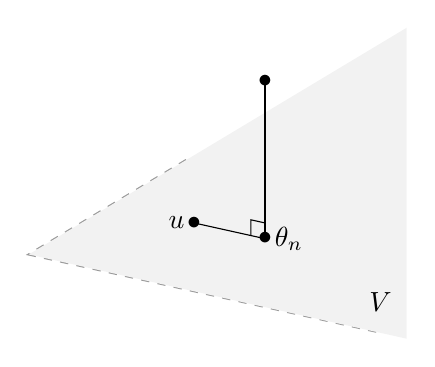
\begin{tikzpicture}[scale=1]%
\draw [dashed, thick, color=gray!80] (2, 2) -- ++(-2, -1.2) -- ++(4.5, -1);%
\fill [color=gray!10] (0, 0.8) -- ++(4.8, 2.88) -- ++(0, -3.95);%
\draw (4.2, 0.2) node[right]{$V$};%
\draw (3, 3) node[right] {$\by$};%
\draw (3, 3) node {$\bullet$};%
\draw (3, 3) -- (3, 1);%
\draw (3, 1) node[right]{$\bX \wh \theta_n$};%
\draw (3, 1) -- ++(-0.9, 0.2);%
\draw (2.1, 1.2) node[left] {$\bX u$};
\draw (2.1, 1.2) node {$\bullet$};
\draw (3, 1) node {$\bullet$};%
\draw (3, 1.2) -- ++(-0.18, 0.04) -- ++(0, -0.2);%
\end{tikzpicture}%
\caption{Geometric explanation of the normal Equation~\eqref{eq:least-squares-normal-equation} where $V = \spa(\bX)$}
\end{marginfigure}%
\begin{equation*}%
	\bX \wh \theta_n = \proj_V (\by),
\end{equation*}
where $\proj_V$ is the orthogonal projection operator onto $V = \{ \bX u : u \in \R^d \} = \spa(\bX) = \spa(X^1, \ldots, X^d)$, the linear space in $\R^n$ which is spanned by the columns of $\bX$.
This means that $\by - \bX \wh \theta_n \perp V$, namely 
\begin{equation*}
	\inr{\bX u, \by - \bX \wh \theta_n} = u^\top \bX^\top (\by - \bX \wh \theta_n) = 0
\end{equation*}
for any $u \in \R^d$, which is equivalent to the so-called \emph{normal equation}
\begin{equation}
	\label{eq:least-squares-normal-equation}
	\bX^\top \bX \wh \theta_n = \bX^\top \by.
\end{equation}
This means that $\wh \theta_n$ is a solution to linear system~\eqref{eq:least-squares-normal-equation}.%
\sidenote{However, from an algorithmic point of view, note that $\wh \theta_n$ is usually \emph{not}  computed by solving the linear system, but instead by using an optimization algorithm to minimize the convex function~$F$.}
Another explanation leading to the same characterization is to use the fact $F$ is convex%
\sidenote{since its Hessian matrix is positive semidefinite: $\grad^2 F(t) = \bX^\top \bX \mgeq 0$}   and differentiable on $\R^d$, so that a minimizer must satisfy the first-order condition $\grad F(t) = 0$ with $\grad F(t) =  2 \bX^\top (\bX t - \by)$, leading again to Equation~\eqref{eq:least-squares-normal-equation}.

At this point, let us recall that the covariance matrix between two random vectors $U$ and $V$ (possibly with different dimensions) such that $\E \norm{U}^2 < +\infty$ and $\E \norm{V}^2 < +\infty$ is given by
\begin{equation*}
	\cov[U, V] = \E \big[ (U - \E U)(V - \E V)^\top \big]
\end{equation*}
and we will denote $\var[U] = \cov[U, U]$ the covariance matrix of $U$.
\marginnote[*-3]{The expectation of a vector (or a matrix) is simply the vector (or matrix) containing the expectation of each random entries.}
Let us also remark that whenever $V = \bA U + b$ for some deterministic matrix $\bA$ and deterministic vector $b$, we have that $\E [V] = \bA \E [U] + b$ and $\var[V] = \bA \var[U] \bA^\top$.

From now on, let us assume that $\E \norm{X}^2 < +\infty$ and that $\E[Y^2] < +\infty$.
This allows to define the $d \times d$ positive semi-definite%
\sidenote{it is a positive semi-definite matrix since we have $u^\top \E[X X^\top] u = \E[u^\top X X^\top u] = \E[  (X^\top u)^2 ] \geq 0$ for any $u \in \R^d$.}
matrix
\begin{equation}
	\E[ X X^\top] = (\E [X_j X_k])_{1 \leq j, k \leq d}.
\end{equation}
We will assume throughout this section that $\E[ X X^\top]$ is invertible, namely that $\E[ X X^\top] \succ 0$.
The next theorem proves that the uniqueness of the least-squares estimator is equivalent to several equivalent properties on the distribution $\P_X$ of~$X$ (the distribution of the features).
\begin{theorem}
	\label{thm:least-squares-existence}
	Assume that $n \geq d$. The following points about $\P_X$ are all equivalent whenever $X_1, \ldots, X_n$ are independent.
	\begin{enumerate}
		\item For any hyperplane $H \subset \R^d$ we have $\P[X \in H] = 0$, namely $\P[X^\top t = 0] = 0$ for any $t \in S^{d-1}$
		\marginnote{where $S^{d-1} = \{ u \in \R^d : \norm{u} = 1 \}$}
		\item $\bX^\top \bX = \sum_{i=1}^n X_i X_i^\top \succ 0$ almost surely
		\item The least squares estimator is uniquely defined and given by
		\begin{equation*}
			\wh \theta_n = (\bX \bX)^{-1} \bX^\top \by
		\end{equation*}
		almost surely.
	\end{enumerate}
	Also, whenever $\P_X$ satisfies either of these points, we say that $\P_X$ is \emph{non-degenerate}.
\end{theorem}

The proof of Theorem~\ref{thm:least-squares-existence} is given in Section~\ref{sec:chap04_proofs} below.
The non-degenerate assumption stated in Point~1 means that $\P_X$ does not put mass on any hyperplane of $\R^d$.
This is a mild assumption: whenever $\P_X \ll \leb$ then this assumption is satisfied, since $\leb[H] = 0$ for any hyperplane $H$.
In the next section, we provide some first statistical properties about the least-squares estimator $\wh \theta_n$, under the assumption that $\P_X$ is non-degenerate.

\section{Properties of the least squares estimator} % (fold)
\label{sec:some_properties_of_the_least_squares_estimator}

In this Section we work under the assumption that $\bX^\top \bX \succ 0$ almost surely (this is Point~2 of Theorem~\ref{thm:least-squares-existence}), namely under the assumption that $\P_X$ is non-degenerate.
So, without loss of generality, and in order to simplify notations, we consider in this section that $\bX$ is deterministic%
\sidenote{If we want to work with random $X_1, \ldots, X_n$ then we just need to replace all expectations by conditional expectation with respect to $X_1, \ldots, X_n$.} 
and such that $\bX^\top \bX \succ 0$, so that $\eps_1, \ldots, \eps_n$ are iid and such that $\E[\beps] = 0$.
Furthermore, we assume that the noise is \emph{homoscedastic}, namely $\var[\eps_i] = \sigma^2 < +\infty$, which means $\var[\beps] = \sigma^2 \bI_n$, or equivalently that the covariance of $\beps$ is \emph{isotropic}.
In this setting, the least-squares estimator is given by $\wh \theta_n = (\bX^\top \bX)^{-1} \bX^\top \by$ so that
\begin{equation}
	\label{eq:mean-ols}
	\E_\theta[\wh \theta_n] = (\bX^\top \bX)^{-1} \bX^\top \E_\theta[\by] = (\bX^\top \bX)^{-1} \bX^\top \bX \theta = \theta
\end{equation}
which means that $\wh \theta_n$ is an \emph{unbiased} estimator. We can write also
\begin{equation}
	\label{eq:var-ols}
	\var_\theta[\wh \theta_n] = \var_\theta[ \bA \by] = \bA \var_\theta[\by] \bA^\top = \sigma^2 \bA \bA^\top = \sigma^2 (\bX^\top \bX)^{-1},
\end{equation}
\marginnote[*-2]{this is because $\var_\theta[\by] = \var_\theta[\bX \theta + \beps] = \var[\beps] = \sigma^2 \bI_n$}%
where we used $\bA = (\bX^\top \bX)^{-1} \bX^\top$.
In particular, this proves that the quadratic risk of $\wh \theta_n$ is given by
\begin{equation*}
	\E_\theta \norm{\wh \theta_n - \theta}^2 = \sigma^2 \tr [(\bX^\top \bX)^{-1}].
\end{equation*}
\marginnote[*-2]{Use $\norm{\wh \theta_n - \theta}^2 = \norm{\wh \theta_n - \E_\theta[\wh \theta_n]}^2$ together with the fact that $\E \norm{Z - \E Z}^2 = \tr (\var[Z])$ for a random vector $Z$ such that $\E \norm{Z}^2 < +\infty$.}%
Given $\wh \theta_n$ we can build the vector $\wh \by$ of \emph{predictions} and the vector $\wh \beps$ of \emph{residuals} given by
\begin{equation*}
	\wh \by := \bX \wh \theta_n \quad \text{and} \quad \wh \beps := \by - \bX \wh \theta_n.
\end{equation*}
Note also that $\wh \by = \proj_V(\by) = \bH \by$ where
\begin{equation*}
	\bH := \bX (\bX^\top \bX)^{-1} \bX^\top	
\end{equation*}
is the projection matrix onto $V$.
This matrix is called the \emph{hat matrix} because of the equation $\wh \by = \bH \by$: it puts a hat on $\by$.
Also, note that
\begin{equation}
	\label{eq:residual-noise-relation}
	\by - \wh \by = (\bI_n - \bH) \by = (\bI_n - \bH) (\bX \theta + \beps) = (\bI_n - \bH) \beps
\end{equation} 
since $\bI_n - \bH$ is the projection matrix onto $V^\perp$ (the orthogonal of $V$ which is of dimension $n-d$ since $\bX$ is full rank) and since $\bX \theta \in V$ so that
\begin{equation*}
	\E_\theta \norm{\by - \wh \by}^2 = \E \norm{(\bI_n - \bH) \beps}^2 = \tr \var[(\bI_n - \bH) \beps] = \sigma^2 (n - d),
\end{equation*}
where we used the fact that $(\bI_n - \bH) (\bI_n - \bH)^\top = \bI_n - \bH$ and $\tr(\bI_n - \bH) = n - d$.
This proves that the estimator
\begin{equation*}
	\wh \sigma^2 := \frac{1}{n - d} \norm{\by - \wh \by}^2 
	= \frac{1}{n - d} \norm{\by - \bX \wh \theta_n}^2
\end{equation*}
is an \emph{unbiased} estimator of $\sigma^2$ known as the least-squares estimator of the variance.

A quantity often used to quantity the \emph{goodness-of-fit} of a linear model is the $R^2$, also known as the \emph{coefficient of determination}.
Assuming that $\bone \in \spa(\bX)$, we have by definition of $\wh \theta_n$ that $\by - \bX \wh \theta_n \perp \bX \wh \theta_n - \bar Y_n \bone$,%
\sidenote{Where $\bar Y_n = n^{-1} \sum_{i=1}^n Y_i$ and $\bone \in \R^n$ is the vector with all entries equal to $1$}
so that
\begin{equation*}
	\norm{\by - \bar Y_n \bone}^2 = \norm{\by - \bX \wh \theta_n}^2 
	+ \norm{\bX \wh \theta_n - \bar Y_n \bone}^2
\end{equation*}
and
\begin{equation*}
	0 \leq R^2 := \frac{\norm{\bX \wh \theta_n - \bar Y_n \bone}^2}{\norm{\by - \bar Y_n \bone}^2} = 1 - \frac{\norm{\by - \bX \wh \theta_n}^2 }{\norm{\by - \bar Y_n \bone}^2} \leq 1,
\end{equation*}
which corresponds to the proportion of the (empirical) variance of $\by$ that is ``explained'' by the least-squares fit.
When $R^2$ is close to $1$, then the linear model fits almost perfectly.%
\sidenote{This is not necessarily good news, because of the problem of overfitting, that will be discussed later.}

Now, if we want to go further, we need some extra structure, in particular if we want to study the distributions of $\wh \theta_n$ and $\wh \sigma^2$. 
To do so, we assume in the next section that the noise vector $\beps$ is Gaussian.

\section{Gaussian linear model} % (fold)
\label{sec:gaussian_linear_model}


We keep the same setting as in Section~\ref{sec:some_properties_of_the_least_squares_estimator} but furthermore assume that $\eps_1, \ldots, \eps_n$ are iid and that $\eps_i \sim \nor(0, \sigma^2)$.
This means that $\beps$ is a Gaussian vector with multivariate Gaussian distribution $\beps \sim \nor(0, \sigma^2 \bI_n)$.
Let us start with some reminders about Gaussian vectors.

\paragraph{Gaussian vectors.} % (fold)

We say that a random vector $Z \in \R^n$ is \emph{Gaussian} whenever $\inr{u, Z}$ is a Gaussian real random variable for any $u \in \R^d$.
In this case, we write $Z \sim \nor(\mu, \bSigma)$ where $\mu = \E[Z]$ and $\bSigma = \var[Z]$.
Moreover, if $\bSigma \succ 0$, then $Z$ has density
\begin{equation*}
	f_Z(z) = \frac{1}{\sqrt{(2 \pi)^d \det \bSigma}} \exp \Big( - \frac 12 (z - \mu)^\top \bSigma^{-1} (z - \mu) \Big)
\end{equation*}
with respect to the Lebesgue measure on $\R^n$.
If $Z \sim \nor(0, \bI_n)$, we say that $Z$ is \emph{standard Gaussian} and note that in this case 
$\bA^{1/2} Z + b \sim \nor(b, \bA)$ for any matrix $\bA \mgeq 0$.
Also, if $Z \sim \nor(\mu, \bSigma)$ where $\bSigma$ is a diagonal matrix, then the coordinates of $Z$ are independent.
Note also that if $Z \sim \nor(0, \bI_n)$ and $\bQ$ is orthonormal then $\bQ Z \sim \nor(0, \bI_n)$.


\subsection{Some classical distributions} % (fold)
\label{sub:some_classical_distributions}

In the section, we give some reminders about classical distributions, that will prove useful for the study of the Gaussian linear model.


\paragraph{Gamma distribution.} % (fold)

The Gamma distribution $\gam(a, \lambda)$, where $a > 0$ is the \emph{shape} and $\lambda > 0$ is the \emph{intensity} has density
\begin{equation*}
	f_{a, \lambda}(x) = \frac{\lambda^a}{\Gamma(a)} x^{a - 1} e^{-\lambda x} \ind{x \geq 0}
\end{equation*}
with respect to the Lebesgue measure on $\R$.
\marginnote[*-2]{Recall that $\Gamma(a) = \int_0^{+\infty} x^{a-1} e^{-x} dx$ for $a > 0$ and that $\Gamma(a+1) = a \Gamma(a)$.}%
If $G \sim \gam(a, \lambda)$ then $\E[G] = a / \lambda$ and $\var[G] = a / \lambda^2$ and $\mode(G) = (a - 1) / \lambda$ if $a > 1$.\sidenote{The mode is defined, whenever it exists, as the argmax of the density. It is therefore a value around which we expect to see most of the observations.}
Whenever $G_1 \sim \gam(a_1, \lambda)$ and $G_2 \sim \gam(a_2, \lambda)$ are independent random variable, then $G_1 + G_2 \sim \gam(a_1 + a_2, \lambda)$.
Also, if $E_1, \ldots, E_n$ are iid distributed as $\exp(\lambda)$ then $\sum_{i=1}^n E_i \sim \gam(n, \lambda)$.

\paragraph{The Chi-squared distribution.} % (fold)

If $n \in \N \setminus \{ 0 \}$ then $\chisq(n) = \gam(n/2, 1/2)$ is called the \emph{Chi-squared distribution with $n$ degrees of freedom}.
Although being an instance of the $\gam$ distribution, the $\chisq(n)$ distribution is particularly useful  in statistics, in particular since it is the distribution of $\norm{Z}^2$ where $Z \sim \nor(0, \bI_n)$. 
This comes from the fact that $Z_i^2 \sim \gam(1/2, 1/2)$ so that by independence $\norm{Z}^2 = \sum_{i=1}^n Z_i^2 \sim \gam(n/2, 1/2) = \chisq(n)$.
The density of $\chisq(n)$ is therefore 
\begin{equation*}
	f_n(x) = \frac{2^{-n / 2}}{\Gamma(n/2)} x^{n / 2 - 1} e^{-x / 2} \ind{x \geq 0}
\end{equation*}
with respect to the Lebesgue measure on $\R$.

\paragraph{The Student's $t$ distribution.} % (fold)

If $U \sim \nor(0, 1)$ and $V \sim \chisq(n)$ are independent random variables, then
\begin{equation}
	\label{eq:student-definition}
	\frac{U}{\sqrt{V / n}} \sim \stu(n)
\end{equation}
where $\stu(n)$ is called the \emph{student distribution with $n$ degrees of freedom}%
\sidenote{The name ``Student'' comes from the use of ``Student'' as a pen name for a research paper by W. William Gosset, a statistician and chemist who worked on stabilizing the taste of the beer at the Guiness factory in Dublin (he used ``Student'' in order to stay anonymous and keep secret the use of the $t$-test at the factory).}
which has density%
\begin{marginfigure}
	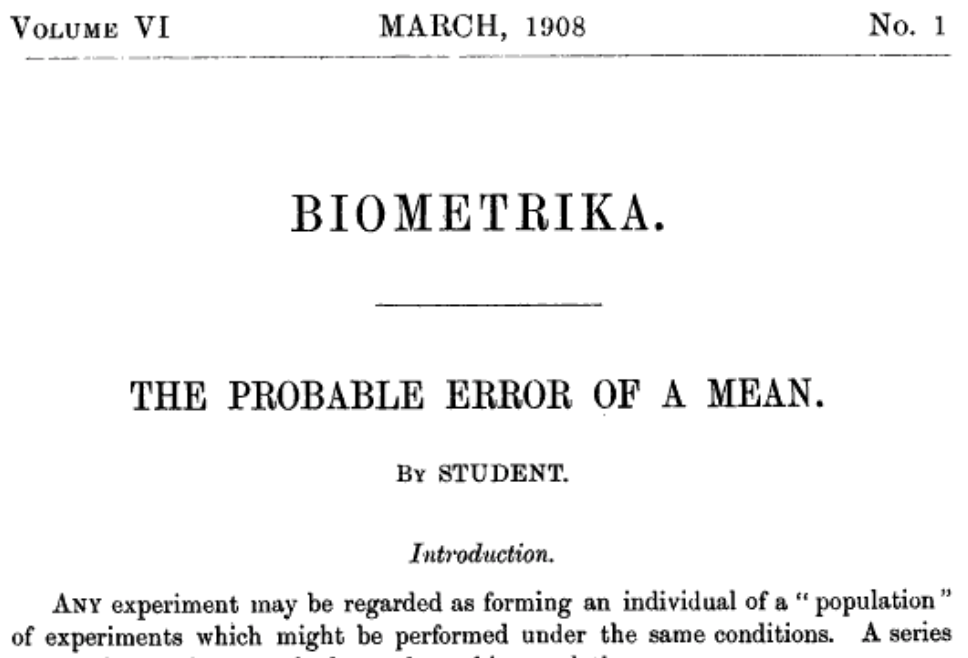
\includegraphics{images/student.png}
\end{marginfigure}
\begin{equation*}
	f_n(x) = \frac{1}{\sqrt{n \pi}} \frac{\Gamma((n+1) / 2)}{\Gamma(n/2)} \frac{1}{(1 + x^2 / n)^{(n + 1)/2}}
\end{equation*}
with respect to the Lebesgue density on $\R$.
If $T \sim \stu(n)$ we have $\E[T] = 0$ and $\var(T) = n / (n - 2)$ whenever $n > 2$.
Also, we have that $\stu(n) \gosto \nor(0, 1)$ as $n \rightarrow +\infty$ since $V / n \gopro 1$ (using the law of large numbers and Theorem~\ref{thm:slutsky}).

% \todo{Insert exercise on the Student distribution}

\paragraph{The Fisher distribution.}

Let $p, q \in \N \setminus \{ 0 \} $. If $U \sim \chisq(p)$ and $V \sim \chisq(q)$ are independent then
\begin{equation}
	\label{eq:fisher-definition}
	\frac{U / p}{V / q} \sim \fis(p, q)
\end{equation}
where $\fis(p, q)$ stands for the \emph{Fisher distribution} with density
\begin{equation*}
	f_{p, q}(x) = \frac{1}{x \beta(p/2, q/2)} \Big( \frac{px}{px + q} \Big)^{p/2} \Big(1 - \frac{px}{px + q} \Big)^{q/2} \ind{x \geq 0}
\end{equation*}
with respect to the Lebesgue measure on $\R$, where
\begin{equation}
	\label{eq:beta-function}
	\beta(a, b) = \frac{\Gamma(a) \Gamma(b)}{\Gamma(a + b)}  = \int_0^1 t^{a-1} (1 - t)^{b - 1} dt.
\end{equation}

\paragraph{The Beta distribution.} % (fold)

If $G_1 \sim \gam(a, \lambda)$ and $G_2 \sim \gam(b, \lambda)$ are independent then
\begin{equation*}
	\frac{G_1}{G_1 + G_2} \sim \bet(a, b)
\end{equation*}
where $\bet(a, b)$ is the Beta distribution with density
\begin{equation*}
	f_{a, b}(x) = \frac{1}{\beta(a, b)} x^{a - 1} (1 - x)^{b - 1} \ind{[0, 1]}(x)
\end{equation*}
with respect to the Lebesgue measure on $\R$, where the $\beta$ function is given by~\eqref{eq:beta-function}.
If $B \sim \bet(a, b)$ then $\E[B] = \frac{a}{a + b}$, $\var[B] = ab / ((a + b)^2 (a + b + 1))$ and $\mode(B) = (a - 1) / (a + b - 2)$ whenever $a, b > 1$.


\subsection{Joint distribution of $\wh \theta_n$ and $\wh \sigma^2$ and consequences}


In order to study the distribution of $\wh \theta_n$ and $\wh \sigma^2$, we need the following theorem, which proves that the projections onto orthogonal spaces of a Gaussian vector with isometric covariance are independent and Gaussian.
\begin{theorem}[Cochran theorem]
	\label{thm:cochran}
	Let $Z \sim \nor(0, \bI_n)$ and let $V_1, \ldots, V_k$ be orthogonal linear spaces of $\R^n$. Define the Gaussian vectors $Z_j = \bP_j Z := \proj_{V_j}(Z)$, where $\bP_j$ is the orthonormal projection matrix onto $V_j$. Then, we have that $Z_1, \ldots, Z_k$ are independent Gaussian vectors, and that
	\begin{equation}
		\norm{Z_j}^2 \sim \chisq(n_j)
	\end{equation}
	where $n_j = \dim(V_j)$ (note that $\sum_{j=1}^k n_j \leq n$).
\end{theorem}
The proof of Theorem~\ref{thm:cochran} is given in Section~\ref{sec:chap04_proofs} below.
Let us go back to the Gaussian linear model where $\by = \bX \theta + \beps$ with $\beps \sim \nor(0, \sigma^2 \bI_n)$.
We know that $\wh \theta_n$ is a Gaussian vector, as a linear transformation of the Gaussian vector $\by$, so that
\begin{equation*}
	\wh \theta_n \sim \nor(\theta, \sigma^2 (\bX^\top \bX)^{-1})
\end{equation*}
in view of Equations~\eqref{eq:mean-ols} and~\eqref{eq:var-ols}.
Moreover, we know from~\eqref{eq:residual-noise-relation} that $\by - \bX \wh \theta_n = (\bI_n - \bH) \beps = \proj_{V^\perp}(\beps)$ and that $\bX (\wh \theta_n - \theta) = \proj_V(\by - \bX \theta) = \proj_V(\beps)$.
Since $V \perp V^\perp$, Theorem~\ref{thm:cochran} entails that $\by - \bX \wh \theta_n$ and $\bX (\wh \theta_n - \theta)$ are independent, so that $\wh \sigma^2$ and $\wh \theta_n$ are also independent.
Moreover, since $\bX$ is full rank, we have $\dim V = d$ and $\dim V^\perp = n - d$, which entails with Theorem~\ref{thm:cochran} that
\begin{equation*}
	(n - d) \frac{\wh \sigma^2}{\sigma^2} = \norm{\proj_{V^\perp}(\beps / \sigma)}^2 \sim \chisq(n-d)
\end{equation*}
and
\begin{equation*}
	\frac{\norm{\bX(\wh \theta_n - \theta)}^2}{\sigma^2 } = \norm{\proj_{V}(\beps / \sigma)}^2 \sim \chisq(n-d).
\end{equation*}
This proves the following theorem.
\begin{theorem}
	\label{thm:gaussian-ols-distribution}
	Assume that $\bX$ is full rank and that $\by = \bX \theta + \beps$ with $\beps \sim \nor(0, \sigma^2 \bI_n)$. Put $\wh \by = \bX \wh \theta_n$ where $\wh \theta_n = (\bX^\top \bX)^{-1} \bX^\top \by$  and $\wh \sigma^2 = \norm{\by - \wh \by}^2 / (n-d)$. 
	Then, we have that $\wh \theta_n$ and $\wh \sigma^2$ are \emph{independent} and such that
	\begin{equation*}
		\wh \theta_n \sim \nor(\theta, \sigma^2 (\bX^\top \bX)^{-1}), \quad (n-d) \frac{\wh \sigma^2}{\sigma^2} \sim \chisq(n - d)
	\end{equation*}
	and $\norm{\bX(\wh \theta_n - \theta)}^2 / \sigma^2 \sim \chisq(d)$.
\end{theorem}

Theorem~\ref{thm:gaussian-ols-distribution} has many consequences for the inference of $\theta$ and $\sigma^2$ in the Gaussian linear model.
If $\sigma^2$ is known, the set
\begin{equation*}
	\cE = \Big \{ t \in \R^d : \frac{1}{\sigma^2} \norm{(\bX^\top \bX)^{1/2} (\wh \theta_n - t)}^2 \leq q_{\chisq(d)}(1 - \alpha)  \Big\}
\end{equation*}
where $q_{\chisq(d)}(1 - \alpha)$ is the quantile function of the $\chisq(d)$ distribution at $1 - \alpha$, is a \emph{confidence set}%
\sidenote{we call also $\cE$ a confidence \emph{ellipsoid}}
for $\theta$ in the Gaussian linear model at level $1 - \alpha$, since it satisfies by construction the coverage property $\P_\theta[ \theta \in \cE] = 1 - \alpha$.
If $\sigma^2$ is unknown (which is always the case), we use the fact%
\sidenote{We proved above that the numerator $\norm{(\bX^\top \bX)^{1/2}(\wh \theta_n - \theta)}^2 / \sigma^2$ has $\chisq(d)$ distribution while the denominator $(n-d) \wh \sigma^2 / \sigma^2$ has $\chisq(n - d)$ distribution and that both are independent, so that the definition~\eqref{eq:fisher-definition} of the Fisher distribution entails the result.}
that
\begin{equation*}
	\frac{\norm{(\bX^\top \bX)^{1/2}(\wh \theta_n - \theta)}^2}{d \wh \sigma^2} \sim \fis(d, n-d)
\end{equation*}
and consider instead the ellipsoid
\begin{equation}
	\label{eq:fisher-ellipsoid-construction}
	\Big \{ \theta \in \R^d : \frac{1}{d \wh \sigma^2} \norm{(\bX^\top \bX)^{1/2} (\wh \theta - \theta)}^2 \leq q_{\fis(d, n - d)}(1 - \alpha)  \Big\},
\end{equation}
which is by construction a confidence set at level $1 - \alpha$.
Note the cute trick involved in~\eqref{eq:fisher-ellipsoid-construction}: the ratio structure allows to cancel out $\sigma^2$, leading to a statistic that does not depend on $\sigma^2$, with a \emph{known} distribution.

% \todo{Y'a quand meme un probleme avec la notation $\theta$. Pourquoi pas $\sigma_0^2$ et en dessous y'en a plus. Faut decider quelque chose}

\paragraph{Confidence intervals.}

Both previous confidence regions provide coverage for the whole vector $\theta \in \R^d$.
We can also build confidence intervals for each coordinate of~$\theta$.
Indeed, we have $\theta_j = \theta^\top e_j$ where $e_j$ is the canonical basis vector with $1$ at coordinate $j$ and $0$ elsewhere. 
More generally, we can build a confidence interval for $a^\top \theta$ for any vector $a \in \R^d$.
We know that $a^\top(\wh \theta_n - \theta) \sim \nor(0, \sigma^2 a^\top (\bX^\top \bX)^{-1} a)$, so that
\begin{equation*}
	\frac{a^\top(\wh \theta_n - \theta)}{\sigma \sqrt{a^\top (\bX^\top \bX)^{-1} a}} \sim \nor(0, 1)
\end{equation*}
and let us recall that $\wh \theta_n$ and $\wh \sigma^2$ are independent and that $(n - d) \wh \sigma^2 / \sigma^2 \sim \chisq(n - d)$.
This entails
\begin{equation}
	\label{eq:ci-construction-gaussian-linear-model}
	\frac{a^\top(\wh \theta_n - \theta)}{\sqrt{\wh \sigma^2 a^\top (\bX^\top \bX)^{-1} a}} 
	\sim \stu(n - d)
\end{equation}
in view of the definition~\eqref{eq:student-definition} of the $\stu$ distribution.%
\sidenote{Note again the fact that the ratio structure in~\eqref{eq:ci-construction-gaussian-linear-model} cancels out $\sigma^2$ and that its \emph{exact} distribution is known, thanks to the assumption that the noise $\beps$ is Gaussian.}
This proves that the interval
\begin{equation*}
	I_{a, 1 - \alpha} = \Big[a^\top \wh \theta_n \pm q_{\stu(n-d)}(1 - \alpha/2) 
	\sqrt{\wh \sigma^2 a^\top (\bX^\top \bX)^{-1} a} \Big],
\end{equation*}
where $q_{\stu(n-d)}$ is the quantile function of the $\stu(n-d)$ distribution,
is a confidence interval for $a^\top \theta$ at level $1 - \alpha$, since it satisfies $\P_\theta[ a^\top \theta \in I_{a, 1 - \alpha}] = 1 - \alpha$ by construction.%
\sidenote{We use the fact that $q_{\stu(k)}(\alpha) = - q_{\stu(k)}(1 - \alpha)$ in this construction, since we know that $\stu(k)$ is a symmetrical distribution in view of~\eqref{eq:student-definition}.}
In particular, for $a = e_j$, we obtain that
\begin{equation}
	\label{eq:ci-gaussian-linear-coordinate}
	\Big[  (\wh \theta_n)_j \pm q_{\stu(n-d)}(1 - \alpha/2) \sqrt{\wh \sigma^2 ((\bX^\top \bX)^{-1})_{j, j}} \Big]
\end{equation}
is a confidence interval for $\theta_j$ at level $1 - \alpha$.

This confidence interval allows to build a test for the hypotheses $H_{0, j} : \theta_j = 0$ versus $H_{1, j} : \theta_j \neq 0$, which can help to quantify the statistical importance of the $j$-th feature in the considered dataset.
Also, a confidence interval for $\sigma^2$ can be easily built using the ancillary statistic $(n - d) \wh \sigma^2 / \sigma^2 \sim \chisq(n - d)$.

\begin{example}
	Consider $Y_1, \ldots, Y_n$ iid $\nor(\mu, \sigma^2)$. This is a Gaussian linear model since $\by = \mu \bone + \beps$ where $\beps \sim \nor(0, \sigma^2 \bI_n)$ and $\bone = [1 \cdots 1]^\top \in \R^n$.
	We have%
	\marginnote{using $(\bone^\top \bone)^{-1} \bone^\top \by = n^{-1} \sum_{i=1}^n Y_i$}
	$\wh \mu_n = \bar Y_n$ together with $\wh \sigma^2 = \frac{1}{n-1} \norm{\by - \bar Y_n \bone}^2 = \frac{1}{n-1} \sum_{i=1}^n (Y_i - \bar Y_n)^2$ and we know from Theorem~\ref{thm:gaussian-ols-distribution} that $\wh \mu_n$ and $\wh \sigma^2$ are independent and such that $\sqrt n (\wh \mu_n - \mu) / \sigma \sim \nor(0, 1)$ and $(n-1) \wh \sigma^2/\sigma^2 \sim \chisq(n-1)$ so that by definition of the $\stu(n-1)$ distribution we have
	\begin{equation*}
		\sqrt{\frac{n}{\wh \sigma^2}} (\wh \mu_n - \mu) \sim \stu(n-1)
	\end{equation*}
	so that we can build, using this ancillary statistic, a confidence interval and tests for $\mu$ when $\sigma^2$ is unknown.
\end{example}

\begin{example}
	Consider the \emph{simple} Gaussian linear regression model where $Y_i = a x_i + b + \eps_i$, with $a, b \in \R$, $x_1, \ldots, x_n \in \R$ and $\eps_i \sim \nor(0, \sigma^2)$ iid. This can be written as a linear model with
	\begin{equation*}
		\by = \bX \theta + \beps =
		\begin{bmatrix}
			1 & x_1 \\
			\vdots & \vdots \\
			1 & x_n
		\end{bmatrix}
		\begin{bmatrix}
			a \\
			b
		\end{bmatrix}
		+ \beps,
	\end{equation*}
	where we can compute explicitly $\wh \theta_n$ and $\wh \sigma^2$ and obtain their distributions using Theorem~\ref{thm:gaussian-ols-distribution}.
\end{example}

\paragraph{Prediction intervals.}

In the previous paragraph, we built confidence sets and intervals for the parameter $\theta \in \R^d$.
But, let us remind ourselves that one of the main usages of the linear model is to provide \emph{predictions} of the label $Y \in \R$ associated to a vector of features $X \in \R^d$.
Once the least-squares estimator $\wh \theta_n$ is computed, we predict the unknown label $Y_{\new}$ of a \emph{new}%
\sidenote{In the sense that $X_{\new}$ does not belong to the dataset $(X_1, Y_1), \ldots, (X_n, Y_n)$ with which $\wh \theta_n$ is trained}
 feature vector $X_{\new} \in \R^d$ using $\wh Y_{\new} = X_{\new}^\top \wh \theta_n$.
If we are willing to assume that the model is Gaussian, namely $\beps \sim \nor(0, \sigma^2 \bI_n)$, and that the unknown label $Y_{\new}$ satisfies the same Gaussian linear model $Y_{\new} = X_{\new}^\top \theta + \eps_{\new}$ where $\eps_{\new}$ is independent of $\beps$ and
 $\eps_{\new} \sim \nor(0, \sigma^2)$, then we know that $\wh Y_{\new}$ and $Y_{\new}$ are independent Gaussian random variables, so that $\wh Y_{\new} - Y_{\new}$ is also Gaussian, and
 $\E_\theta[\wh Y_{\new} - Y_{\new}] = X_{\new}^\top \E_\theta[\wh \theta_n] - X_{\new}^\top \theta = 0$ and
 \begin{align*}
 	\var[\wh Y_{\new} - Y_{\new}] &= \var[\wh Y_{\new}] + \var[Y_{\new}] \\
 	&= \sigma^2 (X_{\new}^\top (\bX^\top \bX)^{-1} X_{\new} + 1),
 \end{align*}
which means that
\begin{equation*}
	\wh Y_{\new} - Y_{\new} \sim \nor\big(0, \sigma^2 (1 + X_{\new}^\top (\bX^\top \bX)^{-1} X_{\new})\big)
\end{equation*}
and using again the fact that $\wh \sigma^2$ and $\wh \theta_n$ are independent and $(n-d) \wh \sigma^2 / \sigma^2 \sim \chisq(n -d)$ we obtain
\begin{equation*}
	\frac{\wh Y_{\new} - Y_{\new}}{\sqrt{\wh \sigma^2  (1 + X_{\new}^\top (\bX^\top \bX)^{-1} X_{\new}) }} \sim \stu(n-d)
\end{equation*}
so that the interval
\begin{align*}
	I_{\new}(X_{\new}) = \Big[ \wh Y_{\new} \pm &q_{\stu(n-d)}(1 - \alpha / 2) \\
	& \times \sqrt{\wh \sigma^2  (1 + X_{\new}^\top (\bX^\top \bX)^{-1} X_{\new}) } \Big]
\end{align*}
is a prediction interval at level $1 - \alpha$, since we have by construction $\P[Y_{\new} \in I_{\new}(X_{\new})] = 1 - \alpha$.


\subsection{The Fisher test} % (fold)
\label{sub:the_fisher_test}

Using the confidence interval~\eqref{eq:ci-construction-gaussian-linear-model} we can test $H_0 = \theta_1 = \theta_2$ by using $a = [1, -1, 0, \ldots, 0]$. 
But, how can we test $H_0 : \theta_1 = \theta_2 = 0$ or more generally a \emph{multiple} null hypothesis such as
\begin{equation}
	\label{eq:fisher-test-multiple-null-example}
	H_0 : \theta_1 = \cdots = \theta_k = 0
\end{equation}
for $k = 2, \ldots, d$ ?
If we fix $j \in \{ 1, \ldots, k\}$ and consider the simple null hypothesis $H_{0, j} : \theta_j = 0$ versus the alternative $H_{1, j} : \theta_j \neq 0$, we know thanks to the confidence interval~\eqref{eq:ci-gaussian-linear-coordinate} together with Proposition~\ref{prop:ci-and-tests} that the test with rejection set 
\begin{equation*}
	R_{j, \alpha} = \Big\{ |(\wh \theta_n)_j| > q_{\stu(n-d)}(1 - \alpha/2) \sqrt{\wh \sigma^2 ((\bX^\top \bX)^{-1})_{j, j}} \Big\}
\end{equation*}
has level $\alpha$, namely $\P_{\theta_j = 0}[R_{j, \alpha}] = \alpha$, for any $j=1, \ldots, k$.
So, an approach to test the multiple hypothesis $H_0$ given by~\eqref{eq:fisher-test-multiple-null-example} would be to consider a rejection set given by the \emph{union} of the individual $R_{j, \alpha}$, with a decreased level $\alpha / k$, since
\marginnote[*2]{The notation $\P_{H_0}$ means that we compute the probability assuming that $H_0$ holds, namely $\theta_1 = \cdots = \theta_k = 0$}
\begin{equation*}
	\P_{H_0} \Big [ \bigcup_{j=1}^k R_{j, \alpha / k} \Big] 
	\leq \sum_{j=1}^k \P_{\theta_j = 0} [ R_{j, \alpha / k} ] \leq k \times \alpha / k = \alpha,
\end{equation*}
so that the test with rejection set $\cup_{j=1}^k R_{j, \alpha / k}$ for the null hypothesis~\eqref{eq:fisher-test-multiple-null-example} has indeed level $\alpha$.
This strategy, which relies on a union bound for the construction of a \emph{multiple test} is called the Bonferroni correction.%
\sidenote{This is called Bonferroni correction, although this strategy is due to Olive Jean Dunn (1915–2008) who worked on statistical testing for biostatistics.}
It is the simplest approach for multiple testing, more about multiple tests will follow later in this book.

This Bonferroni correction requires to replace the individual levels $\alpha$ of each test by the decreased $\alpha /k$, where $k$ is the number of null hypotheses to be tested.
If $k$ is large, this is a large decrease, and we expect a large deterioration of the power of each individual test.
In the Gaussian linear model, we can do much better than this, thanks to the Fisher test.

Let us continue with the null assumption~\eqref{eq:fisher-test-multiple-null-example} and put $\Theta_0 = \{ \theta \in \R^d : \theta_1 = \cdots = \theta_k = 0 \}$. 
Let us that recall that $V = \spa(\bX) = \{ \bX u : u \in \R^d\}$ and introduce $W = \{ \bX u : u \in \Theta_0 \}$. 
Note that $\theta \in \Theta_0$ means that $\bA \theta = 0$ with $\bA = [\bI_k \bO_{k, d-k}]$ corresponding to the horizontal concatenation of the identity matrix on $\R^k$ and a $k \times (d-k)$ zero matrix.
More generally, we can consider a multiple testing problem with null hypothesis
\begin{equation}
	\label{eq:fisher-null-hypothesis}
	H_0 : \theta \in \Theta_0 \quad \text{with} \quad \Theta_0 = \ker(\bA),
\end{equation}
where $\bA$ is a $k \times d$ matrix of rank $k$.
The idea of the Fisher test is to use the fact that $\theta \in \Theta_0$ means that $\bX \theta$ lives in a linear subset $W \subset V$, of dimension $d - k < d$, and to detect statistically this fact.

The Fisher test uses a geometric solution to this testing problem: we decompose $\R^n$ as the following direct sums
\begin{equation*}
	\R^n = V^\perp \oplus V = V^\perp \oplus W \oplus W',
\end{equation*}
where we note that $\dim(V^\perp) = n - d$, $\dim(W) = d - k$ and $\dim(W') = k$, where $W = \{ \bX \theta : \theta \in \Theta_0 \} \subset V$.
Consider now the projections $\proj_V(\by)$ and $\proj_W(\by)$ of $\by$ onto $V$ and its subspace~$W$.
Pythagora's theorem entails that%
\begin{marginfigure}%
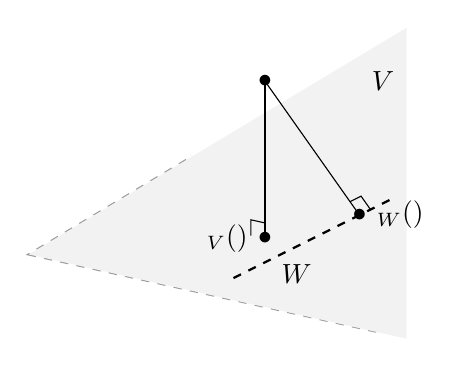
\begin{tikzpicture}[scale=1]%
\draw [dashed, thick, color=gray!80] (2, 2) -- ++(-2, -1.2) -- ++(4.5, -1);%
\fill [color=gray!10] (0, 0.8) -- ++(4.8, 2.88) -- ++(0, -3.95);%
\draw (4.5, 3) node {$V$};%
\draw (3, 3) node[right] {$\by$};%
\draw (3, 3) node {$\bullet$};%
\draw (3, 3) -- (3, 1);%
\draw (3, 1) node[left]{$\proj_V(\by)\;$};%
\draw (3.4, 0.8) node[below] {$W$};
\draw[dashed, thick] (2.6, 0.5) -- ++(2, 1);
\draw (4.2, 1.3) node {$\bullet$};
\draw (4.2, 1.3) node[right] {$\; \proj_W(\by)$};
\draw (4.34, 1.37) -- ++(-0.12, 0.17) -- ++(-0.14, -0.07);
\draw (3, 3) -- (4.2, 1.3);
\draw (3, 1) node {$\bullet$};%
\draw (3, 1.2) -- ++(-0.18, 0.04) -- ++(0, -0.2);%
\end{tikzpicture}%
\caption{Geometric construction of the Fisher test}
\end{marginfigure}%
\begin{equation*}
	\norm{\by - \proj_W(\by)}^2 = \norm{\by - \proj_V(\by)}^2 + \norm{\proj_V(\by) - \proj_W(\by)}^2
\end{equation*}
since $\by - \proj_V(\by) \perp \proj_V(\by) - \proj_W(\by) \in V$, so that 
\begin{equation*}
	\norm{\proj_V(\by) - \proj_W(\by)}^2 = \norm{\by - \proj_W(\by)}^2 - \norm{\by - \proj_V(\by)}^2.
\end{equation*}
Recall that $\proj_V(\by) = \bX \wh \theta_n$ where $\wh \theta_n$ is the least squares estimator while $\proj_W(\by) = \bX \wt \theta_n$ where $\wt \theta_n$ is the least squares estimator computed under $H_0$, namely $\wt \theta_n = \argmin_{\theta \in \Theta_0} \norm{\by - \bX \theta}^2$.
This is where the trick of the test comes into the picture: the quantity $\proj_V(\by) - \proj_W(\by)$ behaves very differently whenever $H_0$ holds or not. 
Indeed, \emph{under $H_0$}, namely when $\bX \theta \in W$, we have
\begin{align*}
	\proj_V(\by) - \proj_W(\by) = \proj_{W'} (\by) &= \proj_{W'}(\bX \theta) + \proj_{W'}(\beps) \\
	&= \proj_{W'}(\beps),
\end{align*}
since in this case $\bX \theta \in W \perp W'$, while $\proj_{W'}(\bX \theta) \neq 0$ when $\theta \notin \Theta_0$.
So, under $H_0$, we have that $(\proj_V(\by) - \proj_W(\by)) / \sigma = \proj_{W'}(\beps / \sigma)$ while 
$(\by - \proj_V(\by)) / \sigma = \proj_{V^\perp}(\beps / \sigma)$. 
Therefore, since $V^\perp \perp W'$, Theorem~\ref{thm:cochran} together with the definition~\eqref{eq:fisher-definition} of the Fisher distribution proves that
\begin{align*}
	\frac{\norm{\proj_V(\by) - \proj_W(\by)}^2 / k}{\norm{\by - \proj_V(\by)}^2 / (n - d)} 
	&= \frac{\norm{\proj_{W'}(\beps / \sigma)}^2 / k}{\norm{\proj_{V^\perp}(\beps / \sigma)}^2 / (n-d)} \\
	&\sim \fis(k, n-d)
\end{align*}
under the $H_0$ hypothesis.%
\sidenote{Theorem~\ref{thm:cochran} tells us that under $H_0$, we have that $\norm{\proj_{W'}(\beps / \sigma)}^2 \sim \chisq(k)$, that $\norm{\proj_{V^\perp}(\beps / \sigma)}^2 \sim \chisq(n - d)$ and that both are independent.}
This can be rewritten, under $H_0$, as 
\begin{align*}
	\frac{\big(\norm{\by - \bX \wt \theta_n}^2 - \norm{\by - \bX \wh \theta_n}^2\big) / k}
	{\norm{\by - \bX \wh \theta_n}^2 / (n - d)} 
	&= \frac{\norm{\bX (\wh \theta_n - \wt \theta_n)}^2}{k \wh \sigma^2} \\
	&\sim \fis(k, n-d).
\end{align*}
Once again, the ratio structure of the ancillary statistic cancels out the unknown $\sigma^2$.
We can conclude now that the Fisher test with rejection region
\begin{equation*}
	R_\alpha = \bigg\{  \frac{\norm{\bX (\wh \theta_n - \wt \theta_n)}^2}{k \wh \sigma^2}  \geq q_{\fis(k, n-d)}(1 - \alpha)  \bigg\}
\end{equation*}
has level $\alpha$ for the null hypothesis~\eqref{eq:fisher-null-hypothesis}, namely that $\sup_{\theta \in \Theta_0} \P_\theta[R_\alpha] = \alpha$.
This test is pretty intuitive and can be understood as follows: if $\theta \in \Theta_0$ then both estimators $\wh \theta_n$ and $\wt \theta_n$ should be close, and $\bX (\wh \theta_n - \wt \theta_n)$ should be, consequently, ``small'', the small miracle being that, in the Gaussian linear model, we can perfectly quantify how small.

\begin{example}
	Consider a Gaussian linear model $Y_i = X_i^\top w + b + \eps_i$ where $w \in \R^{d-1}$, where $b \in \R$ is an intercept%
	\marginnote{In practice, you should always include an intercept in a linear model, unless you have a good reason in not doing so.}
	and the noise $\eps_i \sim \nor(0, \sigma^2)$ is iid. Using the same notations as before, we can rewrite this as $\by = \bX \theta + \beps$ where $\beps \sim \nor(0, \sigma^2 \bI_n)$, where $\theta = [b, w^\top]^\top \in \R^d$ and where $\bX = [\bone X^1 \cdots X^{d-1}]$ is assumed to be full-rank. In this model, we wish to test if the features $X_i$ are useful or if a constant intercept is enough to predict $Y$.
	Namely, we want to test $H_0 : w = 0$ versus $H_1 : w \neq 0$, namely $H_0 : \theta_2 = \cdots = \theta_d = 0$. This can be done using the Fisher test, putting $W = \spa(\bone)$ so that $\dim(W) = 1 = d - k$ with $k = d - 1$ and $\Theta_0 = \{ \theta \in \R^d : \theta_2 = \cdots = \theta_d = 0 \}$. 
	Since $\proj_W(\by) = \bar Y_n \bone_n$, the least-squares estimator under $H_0$ is $\wt \theta_n = \bar Y_n \bone_d$, so that the rejection set at level $\alpha$ of the Fisher test writes in this case 
	\begin{equation}
		\label{eq:linreg-f-test}
		\bigg\{  \frac{\norm{\bX \wh \theta_n - \bar Y_n \bone_n}^2}{(d - 1) \wh \sigma^2}  
		\geq q_{\fis(d-1, n-d)}(1 - \alpha)  \bigg\},
	\end{equation}
	with the same notations as before. The $p$-value of this test can be therefore used as a quantification of how much the features are informative globally to predict the label using a linear model, versus a constant intercept. This test is known as the \emph{$F$-test} for linear regression and the statistic used in~\eqref{eq:linreg-f-test} is known as the \emph{$F$-statistic}.
\end{example}

\subsection{Analysis of variance} % (fold)
\label{sub:analysis_of_variance}

Consider independent random variables $X_{i, j} \sim \nor(m_i, \sigma^2)$ for $i=1, \ldots, k$ and $j=1, \ldots, n_i$, namely, we observe $k$ Gaussian iid samples with respective sizes $n_1, n_2,\dots, n_k$, denoted
\begin{equation*}
	X_{i, \bullet} = [X_{i, 1} \cdots X_{i, n_i}]^\top \in \R^{n_i}.
\end{equation*}
The parameters $m = [m_1 \cdots m_k]^\top \in \R^k$ and $\sigma^2 > 0$ are unknown, and we want to build a test for the hypotheses
\begin{equation*}
  H_0 : m_1 = m_2 = \cdots = m_k  \quad \text{against} \quad H_1 : \exists i \neq i': m_i \neq m_{i'},
\end{equation*}
namely, we want to test if all the samples share the same expectation.
We consider the random vector
\begin{equation*}
	X = [X_{1, \bullet}^\top \cdots X_{k, \bullet}^\top]^\top \in \R^n
\end{equation*}
where $n = \sum_{i=1}^k n_i$, which is the vertical concatenation of the random vectors $X_{1, \bullet}, \ldots, X_{k, \bullet}$.
First, we observe that 
\begin{equation*}
 \mu = \E [X] = 
 \begin{bmatrix}
  m_1 \cdots m_1 \, m_2 \cdots m_2 \cdots m_k \cdots m_k
 \end{bmatrix}^\top \in \R^n
\end{equation*}
belongs to a linear space $E$ of dimension $k$, since $\mu = \sum_{i=1}^k m_i e_i$ where $e_1 \in \R^n$ is the vector with $n_1$ first entries equal to $1$ and the others equal to $0$, $e_2$ the vector with the first $n_1$ entries equal to 0, the next $n_2$ entries equal to $1$ and all others equal to $0$, up to $e_k$ with $n_k$ last entries equal to $1$ and all others $0$, so that $E = \spa(e_1, \ldots, e_k)$ where the $e_i$ are orthogonal.
The orthogonal projection of $X$ onto $E$ is therefore given by
\begin{equation*}
	X_E := \proj_E(X) = \sum_{i=1}^k \frac{1}{n_i} \inr{X, e_i} e_i = \sum_{i=1}^k \bar X_{i, \bullet} e_i
\end{equation*}
where $\bar X_{i, \bullet} := \frac{1}{n_i} \inr{X, e_i} = \frac{1}{n_i} \sum_{j=1}^{n_i} X_{i, j}=$ the average of the $i$-th sample.
The null hypothesis writes $H_0:  \mu \in F$, where $F = \spa(\bone)$ is a linear subspace of $E$ with dimension $1$.
\marginnote{The vector $\bone \in \R^n$ has all its entries equal to $1$.}
The orthogonal projection of $X$ onto $F$ is given by
\begin{equation*}
	X_F := \proj_F(X) = \bar X \bone
\end{equation*}
where $\bar X = \frac 1n \sum_{i=1}^k \sum_{j=1}^{n_i} X_{i, j}$ is the average over all the samples.

We can use the Fisher test to test for $H_0$.
We write $X = \mu + \beps$ where $\beps \sim \nor(0, \sigma^2 \bI_n)$ and decompose 
\begin{equation*}
	\R^n = E^\perp \oplus E = E^\perp \oplus F \oplus W.
\end{equation*}
Let us recall that the idea of the Fisher test is to exploit the fact that $X_E - X_F = X_W = \proj_W(\mu + \beps) = \proj_W(\mu) + \proj_W(\beps)$ and that \emph{whenever $H_0$ is true}, namely $\mu \in F$, we have $\proj_W(\mu) = 0$, so that $\frac{1}{\sigma^2} \| X_E - X_F \|^2 = \| \proj_W( \beps / \sigma) \|^2$. 
Moreover, $X - X_E = \proj_{E^\perp}(X) = \proj_{E^\perp}(\mu + \beps) = \proj_{E^\perp}(\beps)$ since $\mu \in E$ so $\frac{1}{\sigma^2} \| X - X_E \|^2 = \| \proj_{E^\perp}( \beps / \sigma) \|^2$.
Since $\beps / \sigma \sim \nor(0, \bI_n)$ we know from Theorem~\ref{thm:cochran} that
\begin{equation*}
	\| \proj_W( \beps / \sigma) \|^2 \sim \chi^2(k-1) \quad \text{and} \quad
\| \proj_{E^\perp}( \beps / \sigma) \|^2 \sim \chi^2(n-k)
\end{equation*}
since $\dim(E^\perp) = n - k$ and $\dim(W) = k-1$ and that these are independent variables since $E^\perp \perp W$.
This proves that
\begin{equation*}
  T = \frac{\| X_E - X_F \|^2 / (k-1)}{\| X - X_E \|^2 / (n-k)} \sim \fis(k-1, n-k),
\end{equation*}
so we can consider the Fisher test with rejection region 
\begin{equation*}
	R = \{ T \geq q_{\fis(k-1, n-k)}(1 - \alpha) \}.
\end{equation*}
We can rewrite the statistic $T$ in a much more interpretable way.
First, we can write
\begin{align*}
  \| X - X_E \|^2 &= \sum_{i=1}^k \sum_{j=1}^{n_i} (X_{i, j} - \bar X_{i, \bullet})^2 \\
  &= \sum_{i=1}^k n_i  \frac{1}{n_i} \sum_{j=1}^{n_i} (X_{i, j} - \bar X_{i, \bullet})^2 =: n V_{\text{intra}},
\end{align*}
where $V_{\text{intra}}$ is the so-called \emph{intra-class variance}%
\sidenote{A \emph{class} corresponds here to a sample $i$}
which corresponds to the average of the weighted%
\sidenote{weighted by the sample proportions $n_i / n$ for $i=1, \ldots, k$}
 variances $\frac{1}{n_i} \sum_{j=1}^{n_i} (X_{i, j} - X_{i, \bullet})^2$ of each sample  $i=1, \ldots, k$ and second, we have
\begin{equation*}
  \| X_E - X_F \|^2 = \sum_{i=1}^k n_i (\bar X_{i, \bullet} - \bar X)^2 =: n V_{\text{inter}},
\end{equation*}
where $V_{\text{inter}}$ is the \emph{inter-class variance} which corresponds to the weighted variance of the averages of each sample.
This explains the name ANOVA (ANalysis Of VAriance), since the Fisher test uses here the test statistic
\begin{equation*}
  T = \frac{V_\text{inter} / (k-1)}{V_\text{intra} / (n - k)},
\end{equation*}
which is the ratio between the inter and intra-class variances $V_{\text{inter}}$ and $V_\text{intra}$.


\section{Leverages} % (fold)
\label{sec:leverages}

Let us go back now to the general linear model.
We know that the residual vector $\wh \beps = \by - \wh \by = (\bI - \bH) \by$ is such that $\E[\wh \beps] = 0$ and $\var[\beps] = \sigma^2 (\bI - \bH)$, so that
\begin{equation*}
	\wh \beps_i \sim \nor(0, \sigma^2 (1 - h_{i,i})) \text{ where } h_{i, i} = \bH_{i, i} = X_i^\top (\bX^\top \bX)^{-1} X_i.
\end{equation*}
We know that $h_{i, i} \in [0, 1]$ since $\bH$ is an orthonormal projection matrix.%
\sidenote{Using $\bH^2 = \bH$ and $\bH^\top \bH$ we get $h_{i, i} = (\bH^2)_{i, i} = h_{i, i}^2 + \sum_{i' \neq i} h_{i, i'}^2$ so that $h_{i, i} (1 - h_{i, i}) \geq 0$.}
We call $h_{i, i}$ the \emph{leverage score} of sample $i$. We say that $i$ has small leverage whenever $h_{i, i}$ is close to zero while we say that is as a large leverage when $h_{i, i}$ is close to $1$, since in this case the contribution of sample $i$ to the linear model is important, since $\wh \beps_i \approx 0$.
Also, we note that 
\begin{equation*}
	h_{i, i} = \frac{\partial \wh Y_i}{\partial Y_i}
\end{equation*}
since $\wh \by = \bH \by$, namely $\wh Y_i = \sum_{j=1}^d \bH_{i, j} Y_j$.
So, the leverage $h_{i, i}$ can be understood as a quantity that measures the ``self-sensitivity'' to its prediction, namely the influence of $Y_i$ on the computation of $\wh Y_i$.
We will see also in the next Section that the leverage score is a very important concept as it is deeply connected to the \emph{theoretical performance} of the least-squares estimation procedure.
% \todo{Insert studentized residuals ?}

\section{Least squares are minimax optimal} % (fold)
\label{sec:optimality_of_the_least_squares}


While the previous contents is quite classical and well-known, the results provided in this Section are surprisingly recent and coming from the PhD manuscript of J. Mourtada, see~\sidecite{mourtadaphd, mourtada_leastsquares}.

Let us come back to the general case where $(X_1, Y_1), \ldots, (X_n, Y_n)$ are iid with same distribution as $(X, Y)$, with $X \in \R^d$ and $Y \in \R$ such that $\E \norm{X}^2 < +\infty$ and $\E[Y^2] < +\infty$. 
Also, we assume that $\P_X$ is non-degenerate, as explained in Theorem~\ref{thm:least-squares-existence} and we assume that
\begin{equation*}
	\bSigma := \E[X X^\top] \succ 0,
\end{equation*}
namely that $\bSigma$ is invertible.
We consider again the linear model (not Gaussian, the results stated here are much more general than that).
Given $\sigma^2$ and $\P_X$, we consider the following classes of distribution $\P_{X, Y}$ on $(X, Y)$.

\begin{definition}
	We consider the set $\cC(\P_X, \sigma^2)$ of joint distributions $\P_{X, Y}$ such that $X \sim \P_X$ and
	\begin{equation*}
		Y = X^\top \theta^\star + \eps
	\end{equation*}
	for some $ \theta^\star \in \R^d$, where $\eps$ satisfies $\E[\eps | X] = 0$ and $\E[\eps^2 | X] \leq \sigma^2$ almost surely. We consider also the set $\cG(\P_X, \sigma^2) \subset \cC(\P_X, \sigma^2)$ where we assume additionally that $\eps | X \sim \nor(0, \sigma^2)$.
\end{definition}
The set $\cC(\P_X, \sigma^2)$ is a general set of joint distributions on $(X, Y)$ with fixed marginal distribution $\P_X$ and such that $Y$ is a linear function of $X$ plus a noise $\eps$ which is conditionally centered and with finite variance. 
The set $\cG(\P_X, \sigma^2)$ is the same as $\cC(\P_X, \sigma^2)$, but where we assume that $\eps$ is centered Gaussian and independent of $X$.

We consider the quadratic risk
\begin{equation*}
	R(\theta) := \E [ (Y - X^\top \theta)^2] = \int (y - x^\top \theta)^2 \P_{X, Y}(dx, dy).
\end{equation*}
It is easy to see that
\begin{equation*}
	\theta^\star = \argmin_{\theta \in \R^d} R(\theta) = \bSigma^{-1} \E[Y X].
\end{equation*}
Our aim here is to find an estimator%
\sidenote{Namely, a measurable function of $(X_1, Y_1), \ldots, (X_n, Y_n)$.}
$\wh \theta$ of $\theta$  such that the \emph{excess risk}
\begin{equation*}
	\cE(\wh \theta) := R(\wh \theta) - R(\theta^\star)
\end{equation*}
is \emph{minimal}.
Note that if $(X, Y) \sim P$ with $P \in \cC(\P_X, \sigma^2)$, then
\begin{align*}
	\cE(\theta) &= \E [ (Y - X^\top \theta)^2 - (Y - X^\top \theta^\star)^2] \\
	&= \E [ (\theta^\star - \theta)^\top X (2 Y - X^\top (\theta + \theta^\star))] \\
	&= \E [ (\theta^\star - \theta)^\top X (X^\top (\theta + \theta^\star) + 2 \eps)] \\
	&= \E [ (\theta^\star - \theta)^\top X X^\top (\theta + \theta^\star)] \\
	&= \norm{\theta^\star - \theta}_{\bSigma}^2,
\end{align*}%
\marginnote[*-5]{We use here the fact that $Y = X^\top \theta^\star + \eps$ and that $\E[\eps | X] = 0$ almost surely.}%
where we introduced $\norm{x}_{\bSigma}^2 = x^\top \bSigma x$, which is a norm since we assumed $\bSigma \succ 0$.
Whenever $(X, Y) \sim P$ with $P \in \cC(\P_X, \sigma^2)$ we will therefore write
\begin{equation*}
	\cE(\theta) = R(\theta) - R(\theta^\star) = \norm{\theta - \theta^\star}_{\bSigma}^2
\end{equation*}
and whenever $\wh \theta$ depends on the data $(X_1, Y_1), \ldots, (X_n, Y_n)$, we can consider, since $(X, Y)$ is an independent copy with the same distribution,
\begin{equation*}
	\E [ \cE(\wh \theta) ]
\end{equation*}
where this expectation is with respect to $P^{\otimes n}$, for the randomness coming from the data. 
We can consider now the \emph{minimax risk} for a set $\cP$ of distributions:
\begin{equation*}
	\inf_{\wh \theta} \sup_{P \in \cP} \E[\cE(\wh \theta)].
\end{equation*}
The infimum is taken over any possible estimator, namely any statistic of the data, while the sup is over all distributions in $\cP$. Hence the name minimax, since we look at the worst-case excess risk over the considered set $\cP$, but we consider the best possible estimator (with the inf).
Since $\cG(\P_X, \sigma^2) \subset \cC(\P_X, \sigma^2)$, the minimax risk of the former is smaller than the one of the latter.

Some remarks and extra notations are required before we can state the main result of the section.
\begin{itemize}
	\item The linear model is \emph{well-specified} here, since we assume that $Y = X^\top \theta^\star + \eps$ almost surely with $\E[\eps | X] = 0$, so that there is no approximation term of $\E[Y | X]$ by $X^\top \theta^\star$.
	\item For the class $\cP = \cC(\P_X, \sigma^2)$, we expect a \emph{minimax estimator}%
	\marginnote{A minimax estimator is an estimator achieving the minimax risk.}
	 $\wh \theta$ to depend both on $\P_X$ and $\sigma^2$. Quite surprisingly, we will see that it is not the case.
\end{itemize}
Let us introduce
\begin{equation*}
	\wh \bSigma = \frac 1n \sum_{i=1}^n X_i X_i^\top = \frac 1n \bX^\top \bX
\end{equation*}
 and let us introduce also the ``whitened'' random vectors $\wt X_i = \bSigma^{-1/2} X_i$ (so that $\E[\wt X_i (\wt X_i)^\top] = \bI_d$) and define
\begin{equation*}
	\wt \bSigma = \frac 1n \sum_{i=1}^n \wt X_i \wt X_i^\top = \bSigma^{-1/2} \wh \bSigma \bSigma^{-1/2}.
\end{equation*}
The following theorem holds.
\begin{theorem}
	\label{thm:least-squares-minimax}
	Assume that $\P_X$ is non-degenerate, that $n \geq d$ and that $\sigma^2 > 0$. 
	Then
	\begin{equation}
		\label{eq:least-squares-minimax}
		\begin{split}
			\inf_{\wh \theta} \sup_{P \in \cC(\P_X, \sigma^2)} \E [\cE(\wh \theta)] 
			&= \inf_{\wh \theta} \sup_{P \in \cG(\P_X, \sigma^2)} \E [\cE(\wh \theta)] \\
			&= \frac{\sigma^2}{n} \E [\tr(\wt \bSigma ^{-1})].
		\end{split}
	\end{equation}
	Furthermore, the infimum in the minimax risk is achieved by the ordinary least squares estimator~\eqref{eq:least-squares-estimator}.
\end{theorem}

The proof of Theorem~\ref{thm:least-squares-minimax} is done in two steps.
The first step, which proves that the ordinary least squares estimator satisfies the upper bound in~\eqref{eq:least-squares-minimax}, is given in Section~\ref{sec:chap04_proofs} below.
Since the proof of the lower bound requires extra tools from Bayesian statistics, it will be provided in Section~\ref{sec:sec:chap05_proofs} of Chapter~\ref{chap:bayesian_statistics}.

This theorem deserves several remarks.
\begin{itemize}
	\item The theorem proves that the least-squares estimator is, in a fairly general setting, \emph{minimax optimal}: it cannot be improved by another estimator, uniformly over the set of distributions $\cC(\P_X, \sigma^2)$.
	\item The Gaussian noise, namely the class $\cG(\P_X, \sigma^2)$ ``saturates'' the minimax risk, and corresponds to the \emph{least favorable} distribution in the minimax sense.
	\item The minimax risk is invariant by a linear transformation of the features vectors: it is unchanged if one replaces $X_i$ by $X_i' = \bA X_i$ for some deterministic invertible matrix $\bA$. Indeed we have in this case $\wh \bSigma' = \frac 1n \sum_{i=1}^n X_i' X_i'^\top = \bA \wh \bSigma \bA^\top$ so that $(\wh \bSigma')^{-1} \bSigma' = (\bA^\top)^{-1} (\wh \bSigma)^{-1} \bSigma \bA^\top$ which proves that $(\wh \bSigma')^{-1} \bSigma'$ and $(\wh \bSigma)^{-1} \bSigma$ are congruent matrices, so that they share the same trace, namely $\tr((\wh \bSigma')^{-1} \bSigma') = \tr((\wh \bSigma)^{-1} \bSigma)$, and the minimax risk is indeed invariant when replacing $X_i$ by $\bA X_i$. This is of course expected, since the supremum is over linear functions.
\end{itemize}
A lower bound for $\sigma^2 \E [\tr(\wt \bSigma ^{-1})] / n$ can be easily obtained thanks to the following proposition.
\begin{proposition}
	\label{prop:trace-inv-convex}
	The function $\bA \mapsto \tr( \bA^{-1})$ is convex on the cone of positive definite matrices.
\end{proposition}
The proof of Proposition~\ref{prop:trace-inv-convex} is given in Section~\ref{sec:chap04_proofs} below.
By combining Proposition~\ref{prop:trace-inv-convex} and Jensen's inequality, we obtain
\begin{equation*}
	\E [\tr({\wt \bSigma}^{-1}) ] \geq \tr (\E [\wt \bSigma]^{-1} ),
\end{equation*}
but $\E[\wt \bSigma] = \bSigma^{-1/2} \E [\wh \bSigma^{-1}] \bSigma^{-1/2} = \bI_d$, so the lower bound 
\begin{equation*}
	\E [\tr( \wt \bSigma^{-1})] \geq d
\end{equation*}
holds, and consequently the minimax risk satisfies
\begin{equation}
	\label{eq:first-explicit-minimax-lower-bound}
	\inf_{\wh \theta} \sup_{P \in \cC(\P_X, \sigma^2)} \E [\cE(\wh \theta)] 
	= \frac{\sigma^2}{n} \E [\tr(\wt \bSigma ^{-1})] \geq \sigma^2 \frac dn.
\end{equation}

We can also provide another expression for $\E [\tr (\wt \bSigma^{-1})]$ using the leverage scores we discussed in Section~\ref{sec:leverages}.
Let us recall at this point that since $\P_X$ is non-degenerate, and if $X_1, \ldots X_{n+1}$ are iid and distributed as $\P_X$, we have $\sum_{i=1}^{n+1} X_i X_i^\top \succ 0$.
\begin{theorem}
	\label{thm:minimax-leverage}
	Under the same assumptions as that of Theorem~\ref{thm:least-squares-minimax}, the minimax risk can be written as
	\begin{equation*}
		\frac 1n \E [\tr ( \wt \bSigma^{-1}) ] = \E \Big[ \frac{\wh \ell_{n+1}}{1 - \wh \ell_{n+1}} \Big]
	\end{equation*}
	where $\wh \ell_{n+1}$ is the leverage of one data point among $n+1$ given by
	\begin{equation*}
		\wh \ell_{n+1} = X_{n+1}^\top \Big( \sum_{i=1}^{n+1} X_i X_i^\top \Big)^{-1} X_{n+1},
	\end{equation*}
	where $X_1, \ldots, X_n, X_{n+1}$ are iid with distribution $\P_X$.
\end{theorem}

The proof of Theorem~\ref{thm:minimax-leverage} is given in Section~\ref{sec:chap04_proofs} below.
Let us recall that $\wh \ell_{n+1} = \partial \wh Y_{n+1} / \partial Y_{n+1}$ where $\wh Y_{n+1} = X_{n+1}^\top \wh \theta_{n+1}$ where $\wh \theta_{n+1}$ is the ordinary least squares estimator computed on the $n+1$ samples $(X_1, Y_1), \ldots, (X_{n+1}, Y_{n+1})$. 
This theorem entails that the minimax risk, which measures the complexity of the estimation problem,  is completely determined by the leverage score. 
Even more than that, it is the expected value of a convex function of $\wh \ell_{n+1}$, so that the minimax risk is small when $\wh \ell_{n+1}$ is small, and gets larger with a large $\wh \ell_{n+1}$, which is natural since in such a case, the regression problem is more difficult. 

A corollary of Theorem~\ref{thm:minimax-leverage} is an improved lower bound compared to the previous $\sigma^2 d / n$.

\begin{corollary}
	\label{cor:proof-lower-bound-leverage}
	Under the same assumptions as that of Theorem~\ref{thm:least-squares-minimax}, we have that the minimax risk satisfies
	\begin{equation*}
		\frac 1n \E [ \tr ( \wt \bSigma^{-1}) ] = \E \Big[ \frac{\wh \ell_{n+1}}{1 - \wh \ell_{n+1}} \Big] \geq \sigma^2 \frac{d}{n - d + 1}.
	\end{equation*}
\end{corollary}
The proof can be found in Section~\ref{sec:chap04_proofs}.
The lower bound $\sigma^2 d / (n - d + 1)$ is very sharp since it can be seen that
\begin{equation*}
	\E [\cE(\wh \theta_n)] = \sigma^2 \frac{d}{n - d - 1}
\end{equation*}
whenever $\P_X = \nor(0, \bSigma)$, if $\wh \theta_n$ is the ordinary least squares estimator.
This comes from the study of the Wishart distribution, which is the distribution of $\bX^\top \bX$ when $X \sim \nor(0, \bSigma)$.%
\sidenote{We won't pursue further about Wishart distributions.}
This result means that the Gaussian \emph{design} $\nor(0, \bSigma)$ is, almost, the most favorable design for linear regression, since for this distribution, the minimax risk is almost minimal (compare the denominators $n - d - 1$ and $n - d + 1$).%
\sidenote{Finding the most favorable distribution is, up to our knowledge, an open problem. We conjecture that it is given by the uniform distribution on the unit sphere of $\R^d$.}

We were able to provide a lower bound for $\E[ \tr (\wt \bSigma^{-1})]$ that is explicit with respect to $d, n$ and $\sigma^2$.
Now, it remains to provide a similarly explicit upper bound for this quantity.
This requires extra assumptions on $\P_X$.

The first assumption is a ``quantified'' version of the non-degenerate assumption about $\P_X$, see Theorem~\ref{thm:least-squares-existence}. 
Indeed, we assume that there is $\alpha \in (0, 1]$ and $C \geq 1$ such that
\begin{equation}
	\label{eq:quanti-nondegenerate}
	\P[ |X^\top \theta | \leq t \norm{\theta}_{\bSigma} ] \leq (C t)^\alpha
\end{equation}
for any $t > 0$ and any non-zero vector $\theta \in \R^d$. 
This is equivalent to the assumption that $\P[ |\wt X^\top \theta | \leq t] \leq (C t)^\alpha$ for any $\theta \in S^{d-1}$ where we recall that $\wt X = \bSigma^{-1/2} X$.
This assumption ``quantifies'' the assumption $\P[X^\top \theta = 0] = 0$.
The second assumption about $\P_X$ requires that
\begin{equation}
	\label{eq:features-fourth-moment}
	\E [\norm{\bSigma^{-1/2} X}^4] \leq \kappa d^2.
\end{equation}
This is entailed%
\sidenote{Indeed, we have $X^\top \theta = \wt X_j$ for the choice $\theta = \bSigma^{-1/2} e_j$, so that $\E[\wt X_j^4] \leq \E [\wt X_j^2]^2 = \kappa$, where we used $\E[\wt X \wt X^\top] = \bI_d$.
This entails that $\E \norm{\wt X}^4 = \sum_{1 \leq j, k \leq d} \E[ \wt X_j^2 \wt X_k^2] \leq \sum_{j, k} \sqrt{\E[ \wt X_j^4] \E[\wt X_k^4]} \leq \kappa d^2$.}
by the condition $\E[(X^\top \theta)^4]^{1/4} \leq \kappa \E[ (X^\top \theta)^2]^{1/2}$ for any $\theta \in \R^d$.%
\begin{theorem}
	Assume that $X$ satisfies~\eqref{eq:quanti-nondegenerate} and~\eqref{eq:features-fourth-moment} and put $C' = 3 C^4 e^{1 + 9 / \alpha}$. 
	Then, if $n \geq \max(6 d / \alpha, 12 \log(12 / \alpha) / \alpha)$, we have
	\begin{equation*}
		\frac 1n \E \tr [ (\wt \bSigma)^{-1}] \leq \frac dn 
		+ 8 C' \kappa \Big( \frac dn \Big)^2.
	\end{equation*}
	This entails, together with Theorem~\ref{thm:least-squares-minimax} and the lower bound~\eqref{eq:first-explicit-minimax-lower-bound}, that
	\begin{equation*}
		\sigma^2 \frac dn \leq \inf_{\wh \theta} \sup_{P \in \cC(\P_X, \sigma^2)} \E [\cE(\wh \theta)] \leq \sigma^2 \frac dn 
		\Big( 1 + 8 C' \kappa \Big( \frac dn \Big) \Big).
	\end{equation*}
\end{theorem}
The proof of such an explicit upper bound is quite technical and somewhat beyond the scope of this book. It can be found in~\sidecite{mourtada_leastsquares}.

Let us wrap up some of the nice things that we learned in this Section.
\begin{itemize}
	\item Ordinary least-squares are minimax optimal for the well-specified linear regression model. This means that no other statistical procedure can perform (uniformly) better than this simple procedure.
	\item The Gaussian design is almost the most favorable one in the minimax sense.
	\item The minimax rate is exactly of order $\sigma^2 d / n$ under mild assumptions
	 on $\P_X$.
	\item The statistical complexity of the linear regression problem is, when measured by the minimax risk, fully explained by the distribution a leverage scores of one sample among $n+1$.
\end{itemize}


\section{Proofs} % (fold)
\label{sec:chap04_proofs}

\subsection{Proof of Theorem~\ref{thm:least-squares-existence}} % (fold)

Point~(2) $\Leftrightarrow$ Point~(3) is obvious since $\bX^\top \bX \succ 0$ entails that $\bX^\top \bX$ is invertible. 
% Point~(1) $\Leftrightarrow$ Point~(2) is obvious as well, since $0 = \E[X X^\top] u = 0$ entails $0 = u^\top \E[X X^\top] u = \E[ (X^\top u)^2] = 0$ which entails $X^\top u = 0$ almost surely. 
Point~(2) $\Rightarrow$ Point~(1) comes from a proof by contradiction. If $0 < p = \P[X^\top u = 0]$ then $X_i^\top u = 0$ for all $i=1, \ldots, n$ with a probability $p^n > 0$ since $X_1, \ldots, X_n$ are iid, so that $\bX^\top \bX \theta = \sum_{i=1}^n (X_i^\top \theta)^2 X_i = 0$ and $\bX^\top \bX$ cannot be invertible almost surely.
The proof of Point~(1) $\Rightarrow$ Point~(2) can be done by recurrence. 
We first remark that $\bX^\top \bX$ is invertible if and only if $\spa(X_1, \ldots X_n) = \R^d$.%
\sidenote{Indeed, $\ker(\bX^\top \bX) = \ker(\bX)$ so that $\bX^\top \bX u = 0 \Leftrightarrow \bX u = 0 \Leftrightarrow X_i^\top \theta = 0$ for all $i=1, \ldots, n$.}
We will show that $\spa(X_1, \ldots, X_d) = \R^d$ almost surely by recurrence. 
We put $V_k = \spa(X_1, \ldots, X_k)$ so that $\dim(V_k) \leq k \leq d$.
For $k=1$ we do have $\dim V_1 = 1$ so it is OK.
Now, assume that $\dim(V_{k-1}) = k-1$. 
We have that $X_k$ is independent from $V_{k-1} = \spa(X_1, \ldots, X_{k-1})$ and $\dim(V_{k-1}) = k-1 < d$ so that $V_{k-1} \subset H$ where $H \subset \R^d$ is an hyperplane. 
So, we have again by independence that $\P[X_k \in V_{k-1}] = \P[X_k \in V_{k-1} | X_1, \ldots, X_{k-1}] \leq \P[X_k \in H] = 0$ using Point~(1). 
So, $X_k \notin V_{k-1}$ almost surely, and $\dim(V_k) = k$ almost surely. $\hfill \square$


\subsection{Proof of Theorem~\ref{thm:cochran}} % (fold)


We have $\var[Z_j] = \bP_j \bP_j^\top = \bP_j$ since $\bP_j$ is an orthogonal projection matrix and $Z_j = \bP_j Z$, which entails that $Z_j$ is a Gaussian vector%
\sidenote{as a linear transformation of a Gaussian vector}%
and that $Z_j \sim \nor(0, \bP_j)$.
Note that $Z_j$ has no density with respect to the Lebesgue measure, it is a random vector on $\R^n$ which belongs to linear subspace of dimension $n_j < n$. 
Now, we have
\begin{equation*}
	\cov[Z_j, Z_{j'}] = \cov[\bP_j Z, \bP_{j'} Z] = \bP_j \bP_{j'}^\top = \bO
\end{equation*}
\marginnote[*-2]{The matrix $\bO$ stands for the matrix with all entries equal to $0$.}%
since $V_j \perp V_{j'}$, so that $Z_j$ and $Z_{j'}$ are independent random vectors, because 
$[Z_j^\top Z_{j'}^\top]^\top$ is a Gaussian vector with a block diagonal covariance matrix.
This proves that the $Z_1, \ldots, Z_k$ are independent random vectors.
Finally, since $\bP_j$ is an orthogonal projection matrix onto a space of dimension $n_j$, we can decompose it as $\bP_j = \bQ \bD_{n_j} \bQ^\top$ where $\bD_{n_j} = \diag[1, \ldots, 1, 0, \ldots, 0]$ is the diagonal matrix with first $n_j$ diagonal elements equal to $1$ and all others equal to $0$ and where $\bQ$ is an orthonormal matrix.
We know that $Z' := \bQ^\top Z \sim \nor(0, \bI_n)$, so $\bP_j Z = \bQ [Z_1' \cdots Z_{n_j}']^\top =: \bQ Z_-'$ and $\norm{\bP_j Z}^2 = \norm{\bQ Z_-''}^2 = \norm{Z_-''}^2$ (since $\bQ^\top \bQ = \bI_n$), so that finally, we have $\norm{\bP_j Z}^2 = \sum_{j=1}^{n_j} (Z_j')^2$.
This proves that $\norm{\bP_j Z}^2 \sim \chisq(n_j)$ since $Z' \sim \nor(0, \bI_n)$.
$\hfill \square$


\subsection{Proof of Proposition~\ref{prop:trace-inv-convex}} % (fold)
\label{sub:proof_of_proposition_prop:trace-inv-convex}

Put $f(\bA) = \tr(\bA^{-1})$ for $\bA \succ 0$ and consider $\bA, \bB \succ 0$ and $\alpha \in [0, 1]$.
We write
\begin{equation*}
	f(\alpha \bA + (1 - \alpha) \bB) = f(\bA + (1 - \alpha) \bD) = g(1 - \alpha),
\end{equation*}
where we defined $g_{\bA, \bD}(u) = f(\bA + u \bD)$ for $u \in [0, 1]$ and $\bD = \bB - \bA$.
First, let us prove that $g_{\bA, \bD}''(0) \geq 0$ for any $\bA \mgeq 0$ and symmetric $\bD$.
Indeed, we have using a Taylor expansion that
\begin{align*}
	(\bA + \eps \bD)^{-1} &= (\bA (\bI + \eps \bA^{-1} \bD))^{-1} \\
	&= \bA^{-1} - \eps \bA^{-1} \bD \bA^{-1} + \eps^2 (\bA^{-1} \bD)^2 \bA^{-1} + \cdots
\end{align*}
where $\eps > 0$ is small enough and $\cdots$ contains terms of order $O(\eps^3)$.
So, we have that
\begin{align*}
	g_{\bA, \bD}''(0) = 2 \tr( (\bA^{-1} \bD)^2 \bA^{-1} ) 
	% = 2 \tr( \bA^{-1} \bD \bA^{-1} \bD \bA^{-1} ) 
	= 2 \tr( \bC \bA^{-1} \bC^\top)
\end{align*}
where $\bC = \bA^{-1} \bD$.
But $\bA^{-1} \mgeq 0$ so $\bC \bA^{-1} \bC^\top \mgeq 0$ and $g_{\bA, \bD}''(0) \geq 0$.
But
\begin{align*}
	g_{\bA, \bD}''(u) &= \frac{\partial^2}{\partial \eps^2} g_{\bA, \bD}(u + \eps) 
	= \frac{\partial^2}{\partial \eps^2} f(\bA + (u + \eps) \bD) \\
	&= g_{\bA + u \bD, \bD}''(0) \geq 0
\end{align*}
since $\bA + u \bD = (1 - u) \bA + u \bB \mgeq 0$.
This proves that $g_{\bA, \bD} : [0, 1] \rightarrow \R^+$ is convex, which allows to conclude since
\begin{align*}
	f(\alpha \bA + (1 - \alpha) \bB) &= g(1 - \alpha) 
	= g(\alpha \cdot 0 + (1 - \alpha) \cdot 1) \\
	&\leq \alpha g(0) + (1 - \alpha) g(1) \\
	&= \alpha f(\bA) + (1 - \alpha) f(\bB).
\end{align*}


\subsection{Proof of Theorem~\ref{thm:least-squares-minimax}:  the upper bound} % (fold)

This is actually mainly a computation with no particular tricks. 
Recall that $(X, Y)$ is such that $Y = X^\top \theta^\star + \eps$ with $\E[\eps | X] = 0$ and $\E[\eps^2 | X] \leq \sigma^2$.
Thanks to Theorem~\ref{thm:least-squares-existence}, we know that the ordinary least squares estimator $\wh \theta$ satisfies
\begin{align*}
	\wh \theta &= (\bX^\top \bX)^{-1} \bX^\top \by = (\bX^\top \bX)^{-1} \bX^\top (\bX \theta^\star + \beps) \\
		&= \theta^\star + \wh \bSigma^{-1} \frac{1}{n} \sum_{i=1}^n \eps_i X_i
\end{align*}
so that recalling $\inr{u, v}_{\bSigma} =u^\top \bSigma v$ and $\norm{u}_{\bSigma}^2 = \inr{u, u}_{\bSigma}$ we have
\begin{align*}
	\E [\cE(\wh \theta)] &= \E \Big\| \wh \bSigma^{-1} \frac{1}{n} \sum_{i=1}^n \eps_i X_i \Big \|_{\bSigma}^2
	 = \frac{1}{n^2} \sum_{1 \leq i, i' \leq n} \E \langle \wh \bSigma^{-1} \eps_i X_i, \wh \bSigma^{-1} \eps_{i'} X_{i'} \rangle \\
	 &= \frac{1}{n^2} \sum_{1 \leq i, i' \leq n} \E \Big[ \E [ \eps_i \eps_{i'} | X_1, \ldots, X_n] \langle \wh \bSigma^{-1}  X_i, \wh \bSigma^{-1} X_{i'} \rangle \Big].
\end{align*}
But we have $\E [ \eps_i \eps_{i'} | X_1, \ldots, X_n] = 0$ whenever $i \neq i'$ and $\E [ \eps_i \eps_{i'} | X_1, \ldots, X_n] \leq \sigma^2$ whenever $i=i'$. So, we obtain
\begin{align*}
	\E [\cE(\wh \theta)] &\leq \frac{\sigma^2}{n^2} \sum_{i=1}^n \E \norm{\wh \bSigma^{-1} X_i}_{\bSigma}^2 
	= \frac{\sigma^2}{n^2} \sum_{i=1}^n \E \big[ (\wh \bSigma^{-1} X_i)^\top \bSigma \wh \bSigma^{-1} X_i \big] \\
	&= \frac{\sigma^2}{n^2} \sum_{i=1}^n \E \big[ \tr (X_i^\top \wh \bSigma^{-1} \bSigma \wh \bSigma^{-1} X_i) \big]
\end{align*}
since $\tr(x) = x$ for $x \in \R$, so that finally, using the cyclic invariance of the trace and linearity, we obtain
\begin{align*}
	\E [\cE(\wh \theta)] &\leq \frac{\sigma^2}{n^2} \sum_{i=1}^n \E \big[ \tr (\wh \bSigma^{-1} \bSigma \wh \bSigma^{-1} X_i X_i^\top )\big] \\
	&= \frac{\sigma^2}{n} \E \big[ \tr (\wh \bSigma^{-1} \bSigma \wh \bSigma^{-1} \wh \bSigma)\big] \\
	&=\frac{\sigma^2}{n} \E \big[ \tr (\wh \bSigma^{-1} \bSigma)\big] \\
	&=\frac{\sigma^2}{n} \E \big[ \tr ( (\bSigma^{-1/2} \wh \bSigma \bSigma^{-1/2})^{-1}) \big] = \frac{\sigma^2}{n} \E[ \tr (\wt \bSigma^{-1}) ]
\end{align*}
which proves the upper bound. $\hfill \square$


\subsection{Proof of Theorem~\ref{thm:minimax-leverage}} % (fold)


Let $X_{n+1} \sim \P_X$ be independent of $X_1, \ldots, X_n$ and write
\begin{align*}
	\frac 1n \E \tr( \wt \bSigma^{-1}) 
	= \frac 1n \E \tr( (\wh \bSigma)^{-1} \bSigma) 
	= \E \tr( (n \wh \bSigma)^{-1} X_{n+1} X_{n+1}^\top) \\
	= \E \inr{(n \wh \bSigma)^{-1} X_{n+1}, X_{n+1}}.
\end{align*}
The proof uses the following cute trick based on the Sherman-Morrison lemma.

\begin{lemma}[Sherman-Morrison]
	\label{lem:sherman-morrison}
	Let $\bA$ be a $d \times d$ invertible real matrix and $u, v \in \R^d$. Then the following formula holds
	\begin{equation*}
		(\bA + u v^\top)^{-1} = \bA^{-1} - \frac{\bA^{-1} u v^\top \bA^{-1} }{1 + v^\top \bA^{-1} u}.
	\end{equation*}
\end{lemma}
This classical lemma allows to inverse the rank-one perturbation of a matrix as a function of its inverse.
\begin{proof}
	The proof follows from a straightforward computation.
	Put $q = v^\top \bA^{-1} u$ and write
	\begin{align*}
	(\bA + u v^\top) \Big( \bA^{-1} &- \frac{\bA^{-1} u v^\top \bA^{-1}}{1 + v^\top \bA^{-1} u} \Big) \\
	& = (\bA + u v^\top) \frac{\bA^{-1} + q \bA^{-1} - \bA^{-1} u v^\top \bA^{-1}}{1 + q} \\
	&= \frac{\bI + q \bI}{1 + q} = \bI
	\end{align*}
	\marginnote[*-2]{We omit obvious computations here, just develop and cancel the terms...}
	A similar computation shows that 
	\begin{equation*}
		\Big( \bA^{-1} - \frac{\bA^{-1} u v^\top \bA^{-1} }{1 + v^\top \bA^{-1} u} \Big) 
		(\bA + u v^\top) = \bI,
	\end{equation*}
	which proves the claim.
\end{proof}

\begin{lemma}
	\label{lem:sherman-morrison-trick}
 	For any $\bS \succ 0$ and any $v \in \R^d$ we have
	 \begin{equation*}
	 	\inr{\bS^{-1} v, v} = \frac{\inr{(\bS + v v^\top)^{-1} v, v}}{1 - \inr{(\bS + v v^\top)^{-1} v, v}}.
	 \end{equation*}
\end{lemma}
This lemma gives a nice formula that allows to express a quadratic form as a function of its rank-1 perturbation.
\begin{proof}
	We have $\bS + v v^\top \mgeq \bS \succ 0$ so that $\bS + v v^\top$ is invertible and using Lemma~\ref{lem:sherman-morrison} gives
	\begin{equation*}
		(\bS + v v^\top)^{-1} = \bS^{-1} - \frac{\bS^{-1} v v^\top \bS^{-1}}{1 + v^\top \bS^{-1} v},
	\end{equation*}
	so that 
	\begin{align*}
		\inr{(\bS + v v^\top)^{-1} v, v} &= v^\top \bS^{-1} v - \frac{v^\top \bS^{-1} v v^\top \bS^{-1} v}{1 + v^\top \bS^{-1} v} \\
		&= \inr{\bS^{-1} v, v} - \frac{\inr{\bS^{-1} v, v}^2}{1 + \inr{\bS^{-1} v, v}} = \frac{\inr{\bS^{-1} v, v}}{1 + \inr{\bS^{-1} v, v}}
	\end{align*}
	which concludes the proof.
\end{proof}
This proves in particular that $\wh \ell_{n+1} \in [0, 1)$ a.s. since $\wh \bSigma \succ 0$ a.s.
Now, using Lemma~\ref{lem:sherman-morrison-trick}, we obtain
\begin{align*}
	\frac 1n \E [\tr( \wt \bSigma^{-1}) ] &= \E \big[ \inr{(n \wh \bSigma)^{-1} X_{n+1}, X_{n+1}} \big] \\
	&= \E \bigg[ \frac{ \inr{(n \wh \bSigma + X_{n+1} X_{n+1}^\top)^{-1} X_{n+1}, X_{n+1} }}{1 - \inr{(n \wh \bSigma + X_{n+1} X_{n+1}^\top)^{-1} X_{n+1}, X_{n+1} } } \bigg] \\
	&= \E \Big[ \frac{\wh \ell_{n+1}}{1 - \wh \ell_{n+1}} \Big]
\end{align*}
which concludes the proof of Theorem~\ref{thm:minimax-leverage}. $\hfill \square$

\subsection{Proof of Corollary~\ref{cor:proof-lower-bound-leverage}} % (fold)

Theorem~\ref{thm:minimax-leverage} and Jensen's inequality applied with the convex function $x \mapsto x / (1-x)$ on $[0, 1)$ gives
\begin{equation*}
	\E \Big[ \frac{\wh \ell_{n+1}}{1 - \wh \ell_{n+1}} \Big] \geq \frac{\E[\wh \ell_{n+1}]}{1 - \E[\wh \ell_{n+1}]}.
\end{equation*}
Now, an exchangeability%
\sidenote{By ``exchangeability'' we mean that this expectation is unchanged when applying any permutation of $X_1, \ldots, X_{n+1}$, since these are iid.}
argument gives
\begin{align*}
	\E [\wh \ell_{n + 1}] &= \E \bigg[ \Big \langle \Big( \sum_{i'=1}^{n+1} X_{i'} X_{i'}^\top 
	\Big)^{-1} X_{n+1}, X_{n+1} \Big \rangle \bigg] \\
	&= \E \bigg[ \Big \langle \Big( \sum_{i'=1}^{n+1} X_{i'} X_{i'}^\top \Big)^{-1} X_{i}, X_{i} 
	\Big \rangle \bigg]
\end{align*}

for any $i=1, \ldots, n+1$, so that
\begin{align*}
 	\E [\wh \ell_{n + 1}] &= \frac{1}{n+1} \sum_{i=1}^{n+1} \E \bigg[ \Big \langle \Big( \sum_{i'=1}^{n+1} X_{i'} X_{i'}^\top \Big)^{-1} X_{i}, X_{i} \Big \rangle \bigg] \\
 	&= \frac{1}{n+1}  \E \bigg [ \tr \bigg( \Big( \sum_{i=1}^{n+1} X_i X_i^\top \Big)^{-1} \sum_{i=1}^{n+1} X_i X_i^\top \bigg) \bigg] 
 	&= \frac{d}{n + 1},
 \end{align*}
so that
\begin{equation*}
	\E \Big[ \frac{\wh \ell_{n+1}}{1 - \wh \ell_{n+1}} \Big] \geq \frac{d}{n - d + 1},
\end{equation*}
which proves the Corollary $\hfill \square$
